% !TeX root = ../mde-presentation.tex

\subsection*{Federation} \label{sec:federation}

\begin{frame}{Federation} \label{frm:federation}

    A core concept within the model data explorer is the federation between
    multiple MDE instances. This is essential as multiple institutions might
    offer different services for one single dataset. One institution might make
    the data available via THREDDS, the other one might make it available as
    ESRI \lstinline|ImageService|.

    \begin{columns}
        \begin{column}{0.45\textwidth}
            \begin{block}{Core concepts}
                \begin{enumerate}
                    \item Each data groups has a unique hosting MDE
                    \item OAuth for synchronizing user permissions between two MDE instances
                    \item A websocket messaging for synchronizing MDE instances
                \end{enumerate}
            \end{block}
        \end{column}
        \begin{column}{0.45\textwidth}
            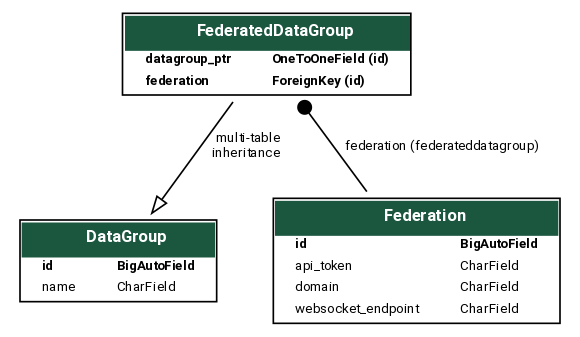
\includegraphics[width=\textwidth]{figures/mde-federation-models.png}
        \end{column}
    \end{columns}

\end{frame}

\begin{frame}{Websocket implementation for federation}

    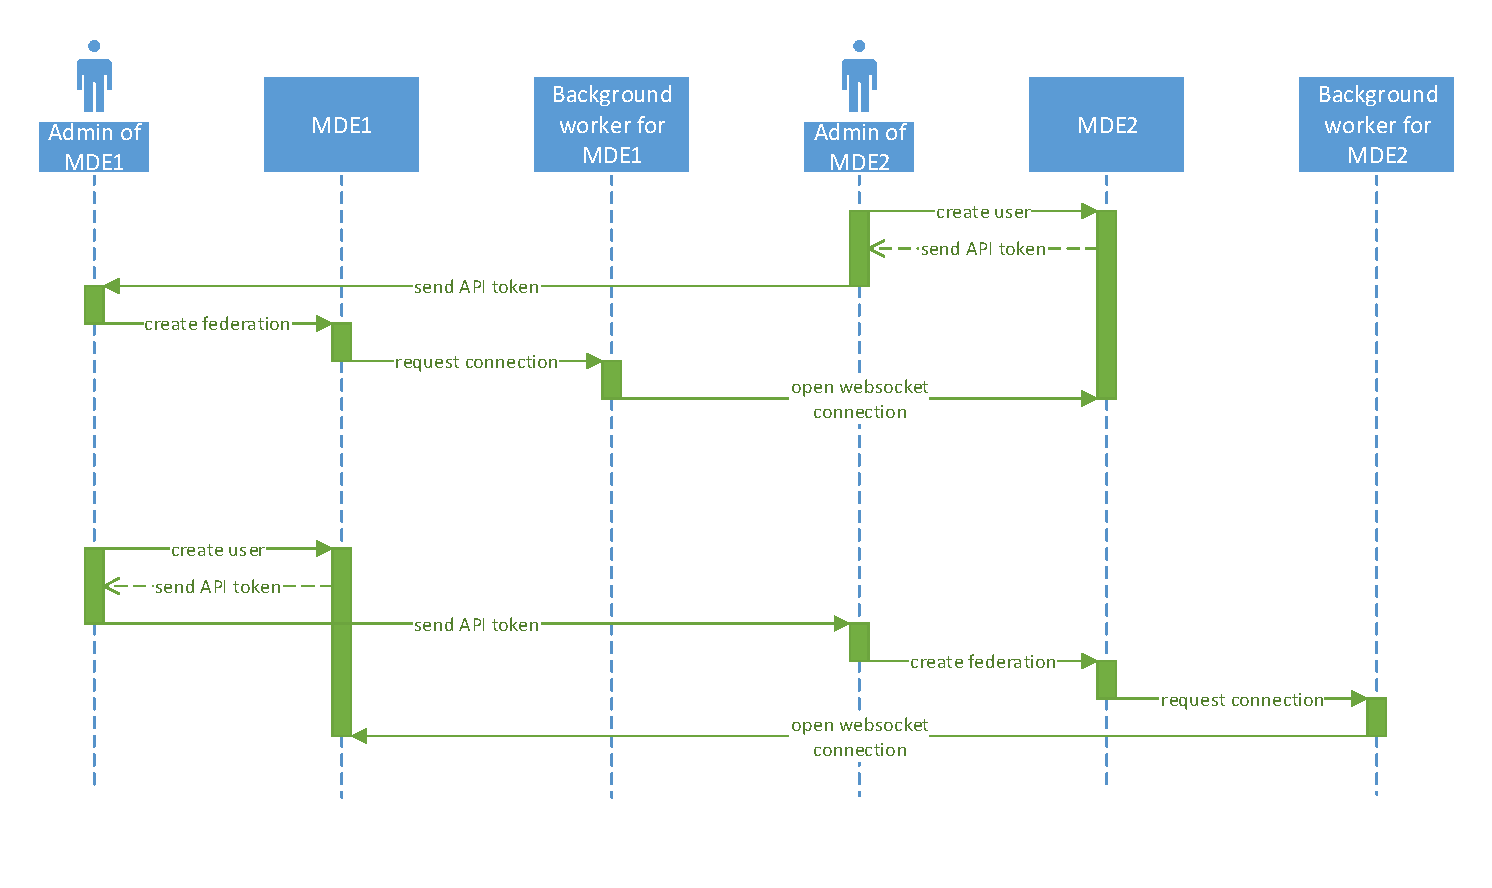
\includegraphics[width=\textwidth]{figures/mde-federation.pdf}

\end{frame}